\documentclass[11pt,a4paper,notitlepage,twocolumn]{article}

\usepackage[T1]{fontenc}
\usepackage[utf8]{inputenc}
\usepackage[english]{babel}
\usepackage{amsmath}
\usepackage{amsfonts}
\usepackage{amssymb}
\usepackage{verbatim}
\usepackage{listings}
\usepackage{color}
\usepackage{setspace}
\usepackage{epstopdf}
\usepackage{graphicx}
\usepackage{caption}
\usepackage{subcaption}
\usepackage{float}
\usepackage{epstopdf}
\usepackage{hyperref}
\usepackage{dsfont}
\usepackage{braket}
\pagenumbering{arabic}
\usepackage{tikz}
\usepackage{fullpage}
\usepackage{titling}

\definecolor{codepurple}{rgb}{0.58,0,0.82}
\definecolor{backcolour}{rgb}{0.95,0.95,0.92}
\definecolor{dkgreen}{rgb}{0,0.6,0}
\definecolor{gray}{rgb}{0.5,0.5,0.5}
\definecolor{mauve}{rgb}{0.58,0,0.82}
%\setlength{\parindent}{0pt}

\lstdefinestyle{pystyle}{
  language=Python,
  aboveskip=3mm,
  belowskip=3mm,
  columns=flexible,
  basicstyle={\small\ttfamily},
  backgroundcolor=\color{backcolour},
  commentstyle=\color{dkgreen},
  keywordstyle=\color{magenta},
  numberstyle=\tiny\color{gray},
  stringstyle=\color{codepurple},
  basicstyle=\footnotesize,  
  breakatwhitespace=false
  breaklines=true,
  captionpos=b,
  keepspaces=true,
  numbers=left,
  numbersep=5pt,
  showspaces=false,
  showstringspaces=false,
  showtabs=false,
  tabsize=2
}
\lstdefinestyle{iStyle}{
  language=IDL,
  aboveskip=3mm,
  belowskip=3mm,
  columns=flexible,
  basicstyle={\small\ttfamily},
  backgroundcolor=\color{backcolour},
  commentstyle=\color{dkgreen},
  keywordstyle=\color{magenta},
  numberstyle=\tiny\color{gray},
  stringstyle=\color{codepurple},
  basicstyle=\footnotesize,  
  breakatwhitespace=false
  breaklines=true,
  captionpos=b,
  keepspaces=true,
  numbers=left,
  numbersep=5pt,
  showspaces=false,
  showstringspaces=false,
  showtabs=false,
  tabsize=2
}
\lstdefinestyle{c++style}{
  language=C++,
  keywordstyle=\color{blue}\ttfamily,
  stringstyle=\color{red}\ttfamily,
  commentstyle=\color{green}\ttfamily,
  morecomment=[l][\color{magenta}]{\#}
  aboveskip=3mm,
  belowskip=3mm,
  columns=flexible,
  basicstyle={\small\ttfamily},
  backgroundcolor=\color{backcolour},
  numberstyle=\tiny\color{gray},
  basicstyle=\footnotesize,  
  breakatwhitespace=false
  breaklines=true,
  captionpos=b,
  keepspaces=true,
  numbers=left,
  numbersep=5pt,
  showspaces=false,
  showstringspaces=false,
  showtabs=false,
  tabsize=2
}
\newcommand{\SE}{Schr\"odinger equation}
\newcommand{\laplacian}{\vec{\nabla}^2}
\newcommand{\eye}{\mathds{I}}
\newcommand\pd[2]{\frac{\partial #1}{\partial #2}}
\def\doubleunderline#1{\underline{\underline{#1}}}


\title{\normalsize Fys3150/4150 - Computational Physics\\
\vspace{10mm}
\huge 5. Continuation on Astronomical project -\\ $N$-body simulation of an open galactic cluster\\
\vspace{10mm}
\normalsize Due date {\bf Nov 9$^{th}$, 2016}}

% Skriv namnet ditt her og fjern kommenteringa
\author{Magnus Christopher Bareid \\ un: magnucb }


\begin{document}
\vspace{5mm}

\begin{titlingpage}
	\begin{center}
    	
\includegraphics[scale=0.5]{../ITA_seal.png}
    	\let\newpage\relax\maketitle

		\begin{figure}[H]
		\center
		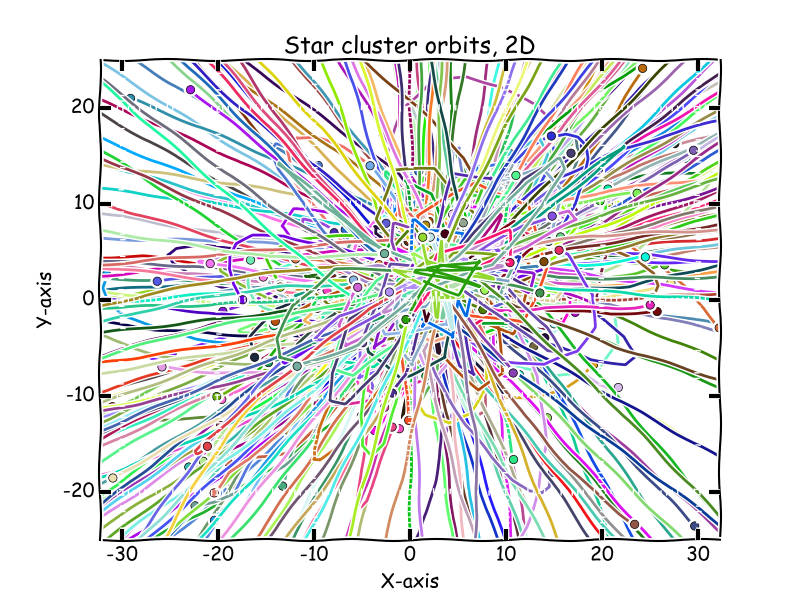
\includegraphics[scale=0.5]{../figs/frontpage.png}
		\end{figure}

		\begin{abstract}
Empty void %TODO
		\end{abstract}

		\newpage
		\tableofcontents

	\end{center}
\end{titlingpage}

%\begin{center}
%\line(1,0){450}
%\end{center}


\newpage

\section*{N-body simulation of an open galactic cluster}
\section{Introduction, or picking up where we left off with the Solar system}
This project is a continuation on a previous project given to the students this semester, in which the students were to gravitationally and numerically simulate the Solar System.

For the current project, the students are to simulate an $N$-body system, unrelated to the Solar system, and investigate properties of the system as it is simulated to reflect on the model's physical validity.

For this purpose, we may review the mathematical equations related to Newtonian gravitation, and other relevant equations.

It is worth noting that the differential integration method we will now utilize, will be the Verlet method, as opposed to the Euler or RungeKutta4 method.

\section{Underlying math}
The most important mathematical expression for an assignment investigating properties of a gravitational system, will be the equations gravitational force exchange.
\subsection{Newton's laws}
The force equation between two objects, will be as per Newton's law of gravity:
\begin{align}\label{eq:gravlaw}
\vec{F}_{G_{i,j}} &= -G\frac{m_i m_j}{r^3_{i,j}}\vec{r}_{i,j}
\end{align}
where $i$ and $j$ denotes which objects' force, in the system of objects' forces, are being measured, the $m$s represents their masses, $r$ is the displacement between the two objects, and $G$ is the Newton's gravitational constant.

Furthermore, Newton's third law of motion comes into place here, as objects are being iterated over, such that
\begin{align}\label{eq:thirdlaw}
\vec{F}_{G_{j,i}} = -\vec{F}_{G_{i,j}}
\end{align}
and the force experienced by the second object of the two equals the same force that the first object experiences, only in the opposite direction.

\subsection{Numerical round-off correction}
At a later point in the project, there is introduced a smoothing factor that helps deal with numerical round-off problems, modifying the force equation thusly:
\begin{align}\label{eq:modgravlaw}
\vec{F}_{G_{i,j}} &= -G\frac{m_i m_j}{r^2_{i,j}+\varepsilon^2}\frac{\vec{r}_{i,j}}{r_{i,j}}
\end{align}
wherein the new quantity $\varepsilon$ represents the aforementioned smoothing factor, with which different magnitudes of values will be experimented.

\subsection{Time and gravitational constant}
Then it is the matter of the system's time scale. It seems arbitrarily that we should measure time in years for a problem that doesn't connect to years in any way. Instead, time is defined through, and normalized by, an analytical expression for an $N$-body system's duration of collapse $\tau_{\text{crunch}}$ (or $\tau_c$ for short), from which we then pull the gravitational constant, dependent on the system's density $\rho_0$, and by extension the cluster's limiting radius $R_0$. The mathematical background and elaboration of $\tau_c$ is based on a topic of cosmology referred to as the "Spherical Top Hat Model" %TODO
, but its formalism is aready given in the project's details.

\begin{align}\label{eq:tauc_and_G}
\tau_c &= \sqrt{\frac{3\pi}{32G\rho_0}} \nonumber \\
\Rightarrow G &= \frac{3\pi}{32\tau_c^2\rho_0}\ , \nonumber \\
\rho_0 &= \frac{\sum_{i} m_i}{\frac{4}{3}\pi R_0^3}\ , \nonumber \\
\Rightarrow G &= \frac{1}{8}\frac{\pi^2 R_0^3}{\tau_c^2 \sum_{i} m_i}\nonumber \\
\intertext{however, as we measure time as an iterated increment of $\tau_c$, its value is normalized to 1, yielding:}\nonumber \\
G &= \frac{1}{8}\frac{\pi^2 R_0^3}{\sum_{i} m_i}
\end{align}


\section{Programming}
The previous project utilized some small-scale general relativity, which at the scales of this current project is obsolete. Instead, the force equation is rewritten according to equation \ref{eq:gravlaw} and \ref{eq:modgravlaw}.

The layout of the class structures largely remain the same, and the main program basically runs the same way, with a few changes.

\subsection{Update of main}
Command line functionality is modified to take in the system's number of bodies \textbf{N}, a time step size \textbf{dt}, correction factor $\varepsilon$, and duration of the simulation.

Next is the random number generation modules initialization, with a uniform distribution of positions for the cluster's stellar bodies, and a gaussian distribution of mass between the stellar bodies, with a mean of 10 Solar masses and a standard deviation of 1 Solar mass.

The cluster's instance is then initialized with a given value for $\varepsilon$, as the calculation of forces and energies betwen stellar bodies is a function of this class.

The stellar bodies now need to be created. To ensure that the cluster's bodies are created in a spherically uniform distribution, the coordinates system in which they are firstinitialized is spherical, and then these are translated into cartesian coordinates. The bodies are then created with a gaussially randomized mass value as described prior.

Now that the cluster's total mass is measured, the gravitational constant $G$ is initialized as per equation \ref{eq:tauc_and_G}, the datafile is opened and the numerical integration begins, producing the clusters' bodies' movement and energies unto the data.

\subsection{Update of Velocity Verlet}
As stated previously, the numerical integrator of the system utilizes the Velocity Verlet method. It should be noted that the previous project's utilization of this algorithm was extremely crudely implemented. For the purpose of this project, however, the algorithm has been cleaned up:
\lstset{style=c++style}
\begin{lstlisting}
void Verlet::integrateOneStep(Cluster &system){
system.calculateForcesAndEnergy();
// Velocity Verlet
for (CelestialBody &body :system.bodies()) {
  // half-step computation
  body.velocity += (m_dt/2.0)*(body.force / body.mass);
  body.position += body.velocity*m_dt;
}
system.calculateForcesAndEnergy();
for (CelestialBody &body :system.bodies()) {
  // the new velocity
  body.velocity += (m_dt/2.0)*(body.force / body.mass);
}}
\end{lstlisting}

This improvement of the code yields an efficiency boost at about 30\%  less time for a standard run of the program with 100 stellar bodies and 4000 time steps to iterate.

\subsection{Time steps}
For the initial test runs of the program, the initial parameters were set to $\mathbf{N} = 100$ stellar bodies, $\mathbf{R_0} = 20$ light years for the stellar bodies' radial distribution's upper displacement limit, and a time resolution of $\mathbf{dt} = 0.001\tau_c$, just to start off.


\section{Appendix}
\subsection{Code and GitHub}
All my code is located at this address:

\url{https://github.com/magnucb/p5}

\begin{thebibliography}{9}
\bibitem{example_code}
  Jensen, M 2016,
  \verb|CodeName|,
  
  viewed $something^{th}$ of December 2016,
  \url{URL}.
  
\bibitem{analytical_methods}
	Jensen, M 2016, 
	Computational Physics Lecture Notes Fall 2015:
	
	13.2.2: Canonical Ensemble \& 
	
	13.3.1: Ising Model and Phase Transitions in Magnetic Systems,
	
	viewed $something^{th}$ of December 2016, 
	\url{URL}

\end{thebibliography}

\end{document}